\documentclass[10pt]{article}
\usepackage{amssymb,amsmath,times,url,graphicx,amsthm,alltt}
%\usepackage[pdftex,urlcolor=blue,pdfpagemode=none,pdfstartview=FitH]{hyperref}
\usepackage{my_packages}
\usepackage{tikz_packages}
\usepackage{wasysym}
%% url smaller font.
\makeatletter
\def\url@leostyle{%
  \@ifundefined{selectfont}{\def\UrlFont{\sf}}{\def\UrlFont{\small\ttfamily}}}
\makeatother
\urlstyle{leo}

%\usepackage[all,import]{xy}

\renewcommand{\baselinestretch}{1.2}
\date{}

\renewcommand{\thesubsection}{\arabic{subsection}. }
\renewcommand{\thesubsubsection}{\arabic{subsection}.\arabic{subsubsection} }

\theoremstyle{definition}
\newtheorem{prob}{Problem}[section]
%\renewcommand{\theprob}{\arabic{section}.\arabic{prob}}
\renewcommand{\theprob}{\arabic{prob}}

\newenvironment{subprob}%
{\renewcommand{\theenumi}{\alph{enumi}}\renewcommand{\labelenumi}{(\theenumi)}\begin{enumerate}}%
{\end{enumerate}}%

\newenvironment{matlab}
{\begin{alltt}\small\renewcommand{\baselinestretch}{1.2}\selectfont}%
{\end{alltt}}


\begin{document}



\setcounter{page}{1}
\pagestyle{plain}
\section*{MAE3145: Homework 6}
\vspace*{-0.4cm}
\noindent{Due date: TBD}%\\%\vspace*{0.5cm}

\begin{prob}
    Neptune is now the furthest ``planet'' in our solar system (since Pluto is classified as a dwarf planet).
    Voyager 2 passed by Neptune in 1989 but there have not been other spacecraft missions to Neptune.
    Consider a Neptune mission by doing a few preliminary calculations. 

    \begin{subprob}
        \item Begin by examining a Hohmann transfer from the Earth to Neptune.
        Assume that planetary orbits are coplanar and circular.
        Compute the total \( \norm{\Delta \vec v_T} \) and the TOF (time of flight in years).
        Ensure you draw proper vector diagrams, and compute \( \norm{\Delta \vec v}\) and \( \alpha \) for each maneuver.
    \item What is \( \norm{\Delta \vec v_1} \), i.e. the maneuver necessary at Earth departure?
        What is \( \norm{\Delta \vec v_2}\) to remain in the Neptune system?
    \item Discuss the feasibility of this mission.
        Is the total cost (\( \norm{\Delta \vec v_T}\)) ``a lot''?
        Is the time of flight reasonable?
        Even though the Hohmann transfer is the minimum two-impulse transfer, is it likely that we could use this transfer to get to Neptune?
    \item Compare the time of flight you calculated to the actual Voyager 2 transfer. 
        You can use the Julian date functions, \texttt{time.date2jd(yr, mo, day, hr, min, sec)}.
    \item Compute the phase angle required at departure for this circle-to-cirle transfer as seen in the heliocentric view.
    \end{subprob}

    \begin{figure}[htbp]
        \centering
        \subcaptionbox{Voyager 2 Image of Neptune\label{fig:neptune}}{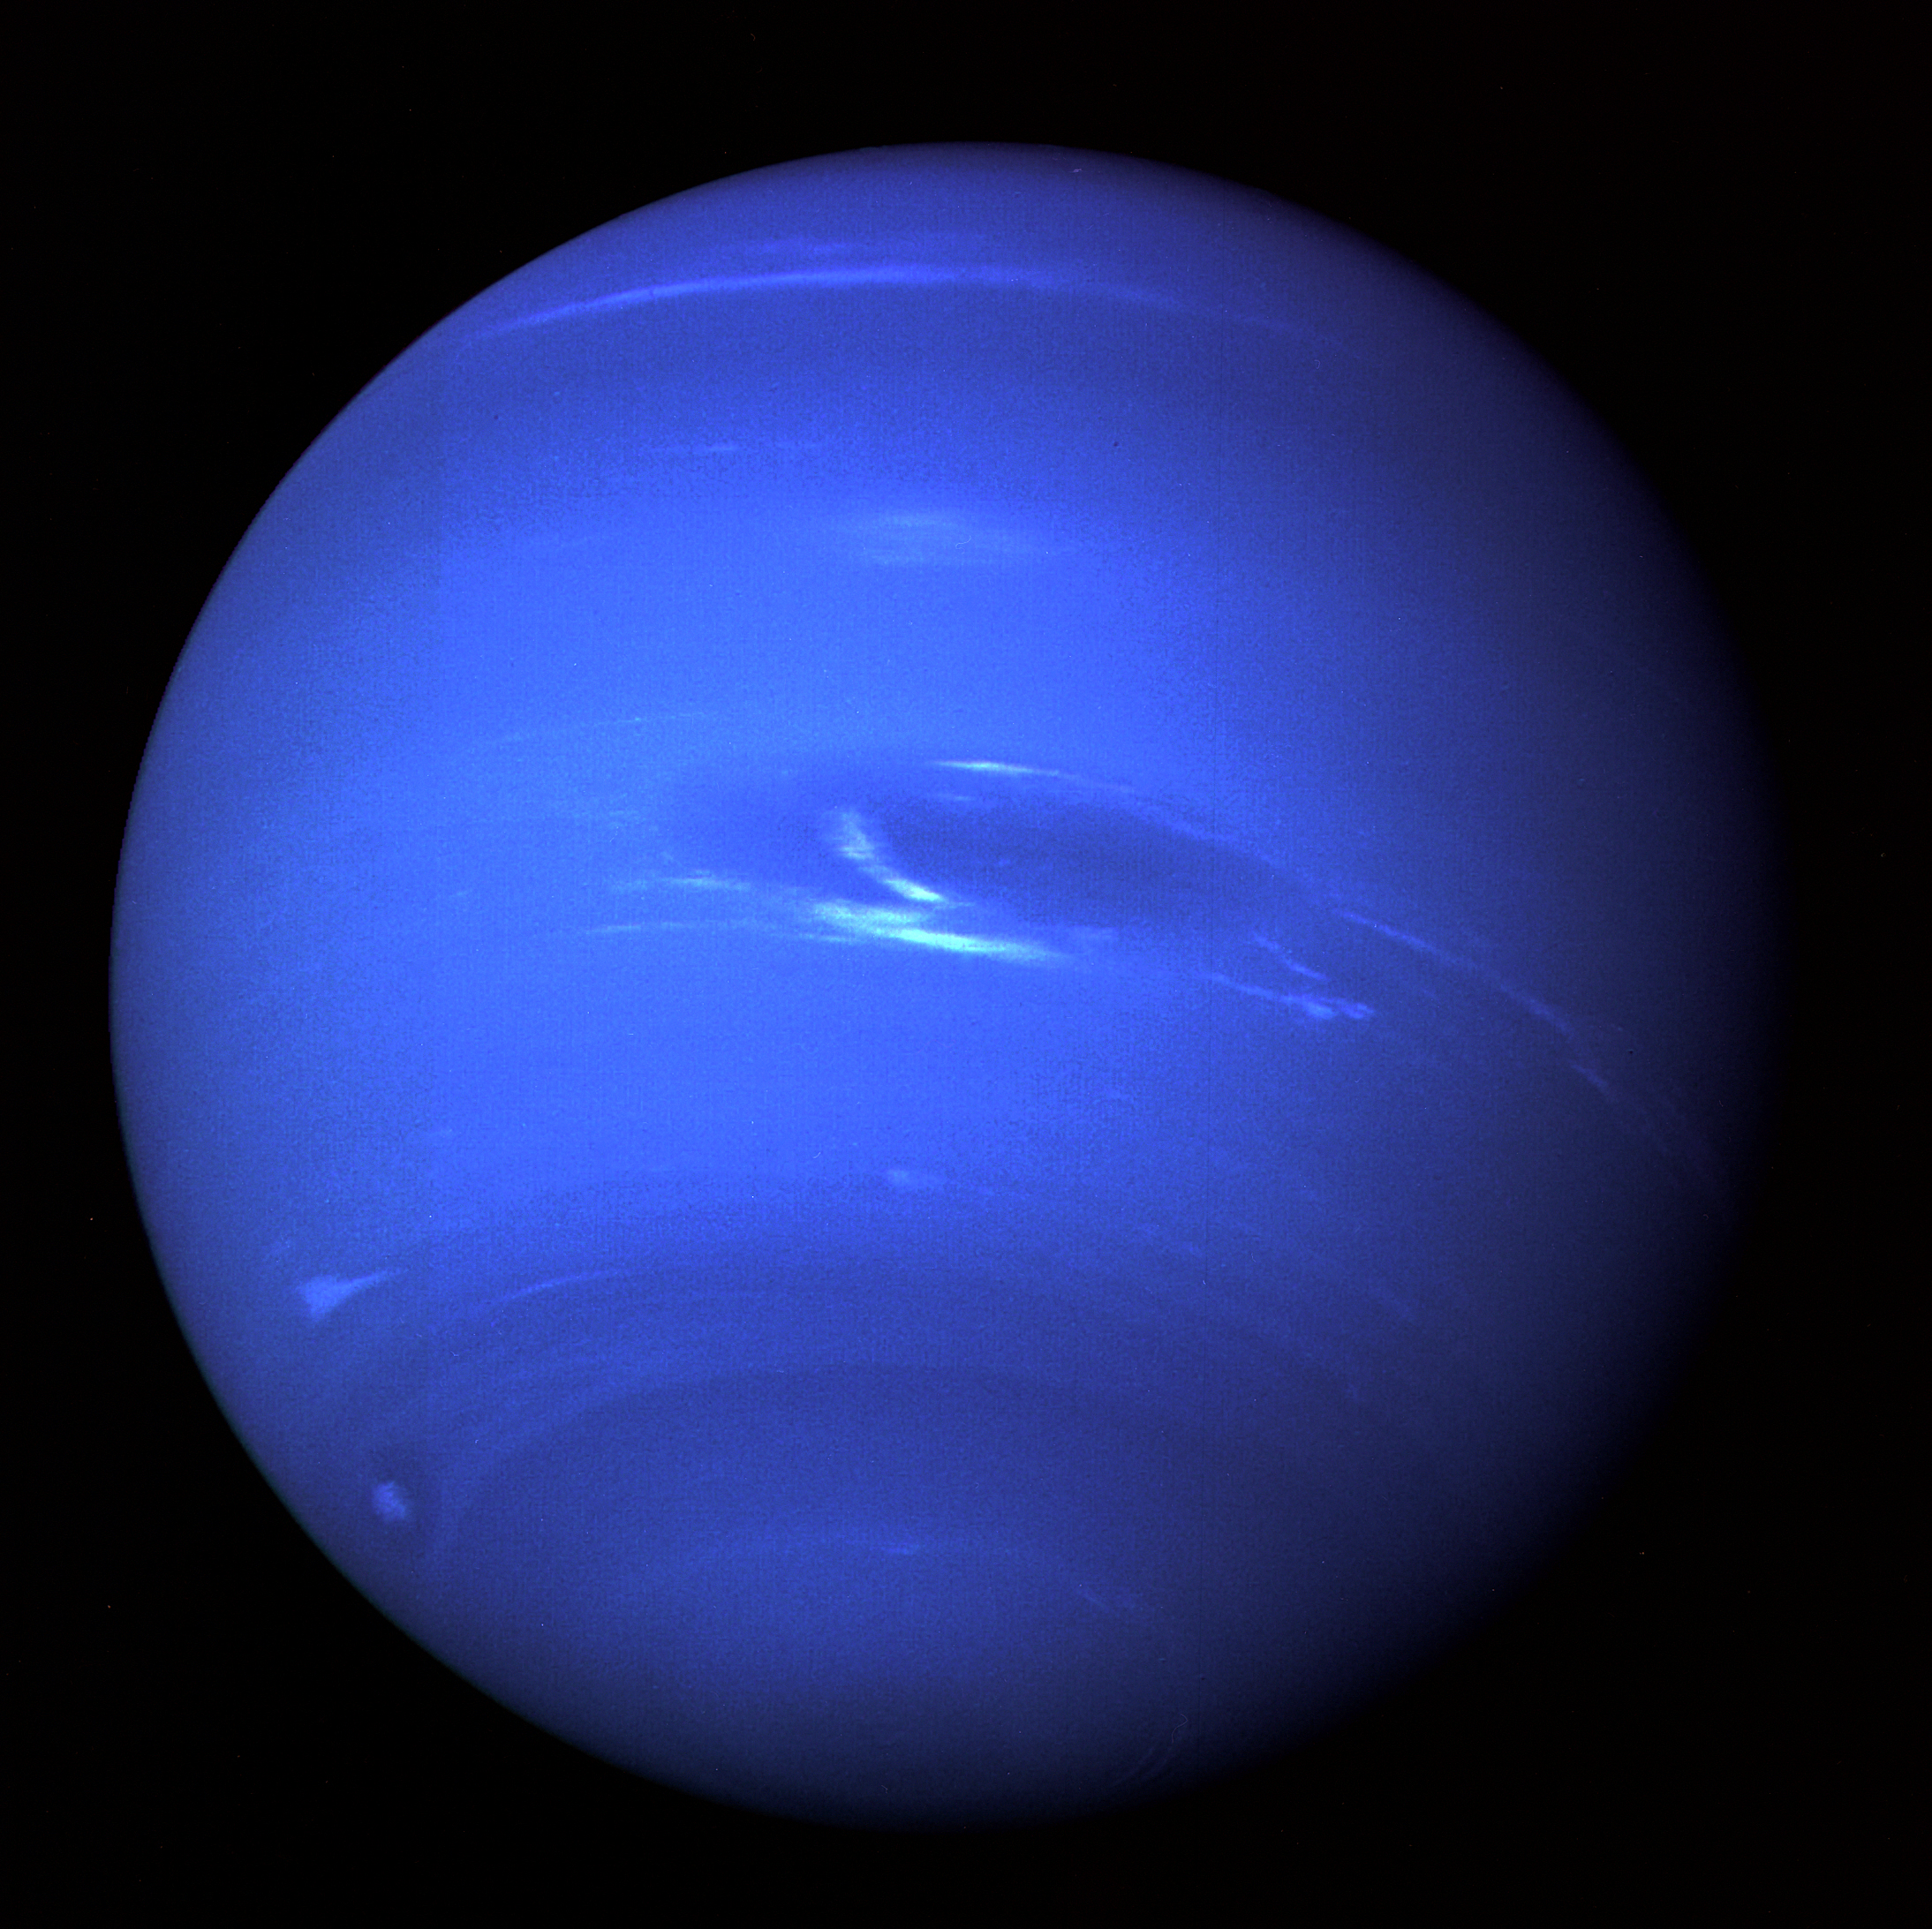
\includegraphics[width=0.5\textwidth]{figures/imageneptune_full.jpg}}~
        \subcaptionbox{Voyager 2 Trajectory\label{fig:voyager2_traj}}{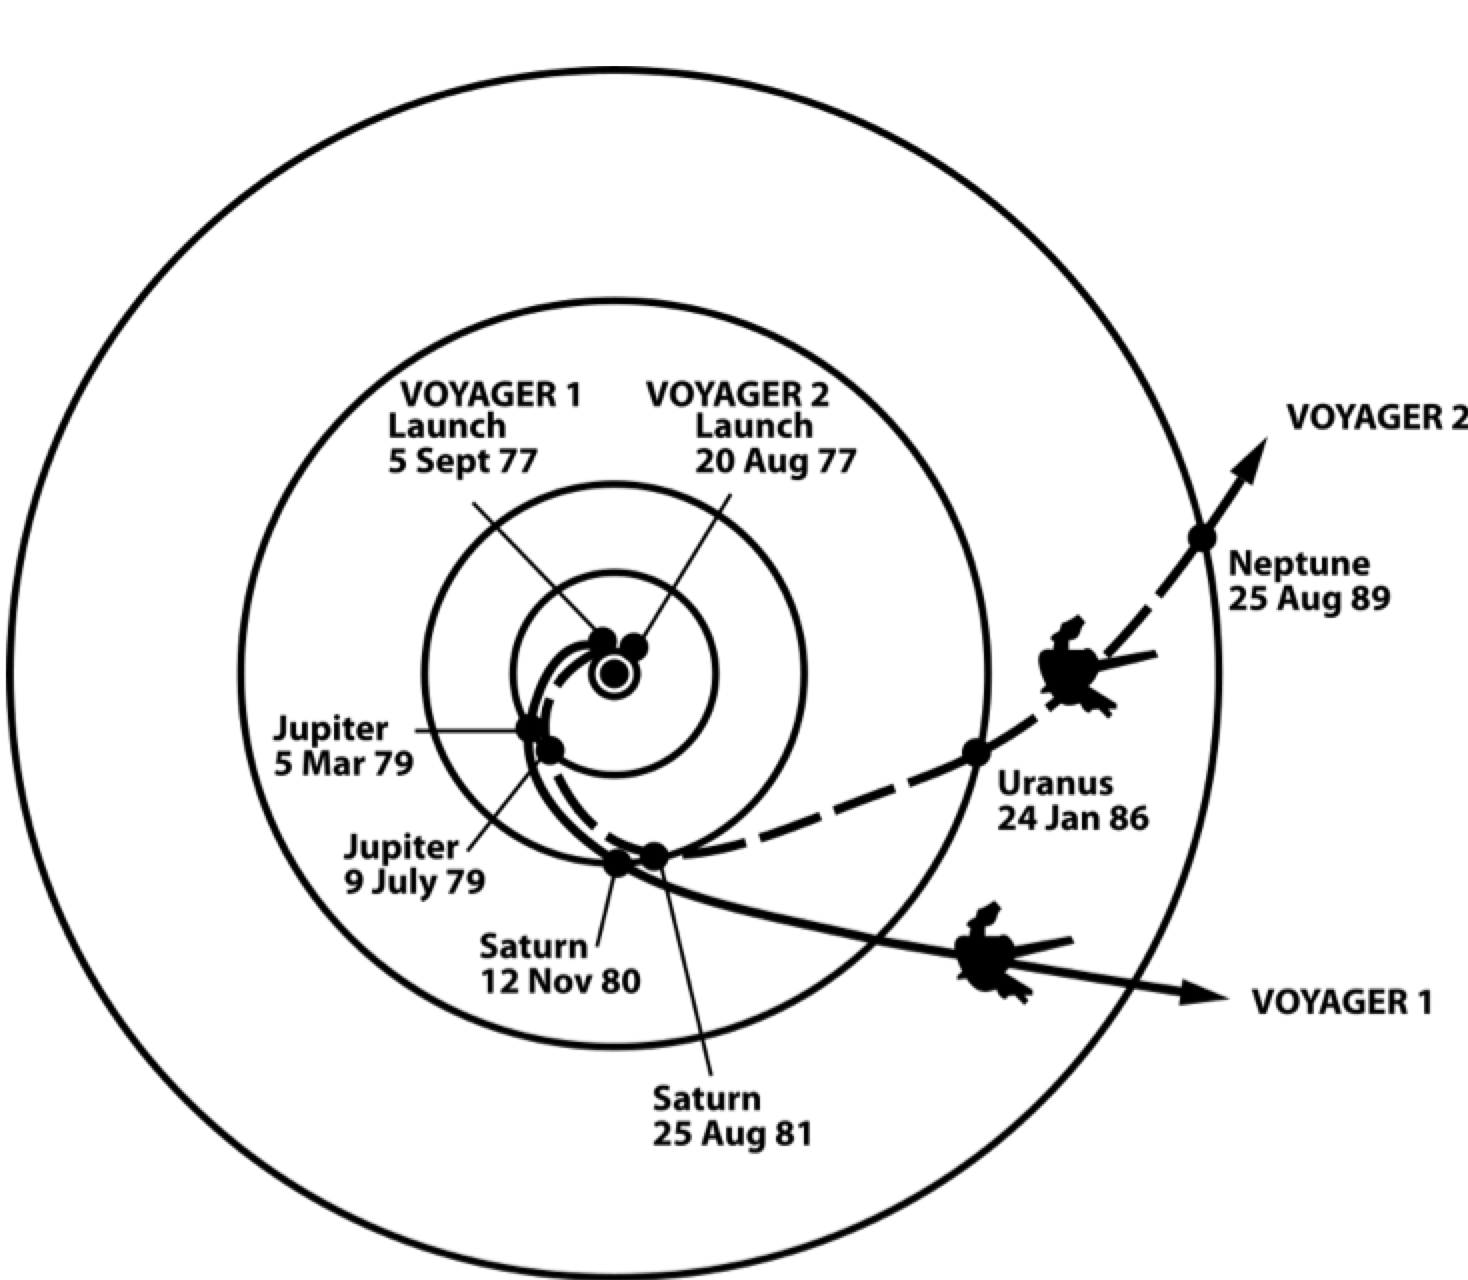
\includegraphics[width=0.5\textwidth]{figures/VoyPlanetTraj.png}}
        \caption{Voyager 2~\label{fig:voyager2}}
    \end{figure}
\end{prob}

\clearpage\newpage
\begin{prob}
    In NASA's original plan for a crewed lunar base (Orion), a ground facility near the Moon's south pole was envisioned, necessitating a polar orbit.
    The lunar south pole offers areas of continual sunlight, which are ideal locations for continuous power generation, the so called ``peaks of eternal light''.
    Thus, the trajectory design ( both arrival at the Moon and the Earth return) included a \SI{90}{\degree} plane change.
    Consider the plane change maneuver. 
    Assume that the spacecraft arrives in the plane of the lunar equator and is currently in a circular orbit at \SI{100}{\kilo\meter} altitude.
    Two options existed for the plane change to the polar orbit.
    \begin{enumerate}
        \item A single maneuver at the current altitude to shift the orbit to an inclination of \SI{90}{\degree}.
        \item A bi-elliptic strategy that includes three maneuvers: A maneuver to raise apoapsis to \SI{17000}{\kilo\meter}, followed by a plane change maneuver at apoapsis, and a final maneuver to insert back into the \SI{100}{\kilo\meter} altitude polar orbit.
    \end{enumerate}

    \begin{subprob}
    \item Compute and compare the cost, i.e. \( \norm{\Delta \vec v} \), for a \SI{90}{\degree} plane change accomplished with the two approaches.
        Assume the single plane change is accomplished instantaneously. 
    \item How much time (TOF) is devoted to the completion of the bi-elliptic option? 
        How does this compare with the single maneuver at the current altitude.
    \end{subprob}
\end{prob}

\begin{prob}
    A vehicle is launched successfully into an orbit with \( e = 0.4\) and \( a = 6 R_{\oplus} \).
    A single in-plane maneuver will be implemented when \( \nu = \SI{90}{\degree}\) (true anomaly).
    Let the maneuver be defined as \( \norm{\Delta \vec v} = \SI{0.75}{\kilo\meter\per\second}\), and \( \alpha = -\SI{60}{\degree}\).

    \begin{subprob}
    \item Express the \( \Delta \vec v \) in terms of the rotating local vertical/local horizontal frame (\( \hat r, \hat \theta \)), perifocal frame (\( \hat p, \hat q \)), and VNC reference frames (\(\hat v, \hat c \)).
    \item Determine the \( r, v, \gamma \) in the new orbit immediately after the maneuver.
        Also compute the following characteristics of the new orbit:
        \begin{align*}
            a \quad e \quad \mathbb{P} \quad \mathcal{E} \quad r_p \quad r_a \quad \nu \quad E \quad (t - T) \quad p \quad \Delta \omega 
        \end{align*}
        Ensure you include a proper vector diagram.
    \item Generate a plot of both the old and new orbits.
        Mark on your plot the vector diagram associated with this maneuver.
    \item As an alternative, wait until the vehicle reaches the end of the minor axis and is descending and then implement the same manuever.
        What is the ``wait time'' to travel from \( \nu = \SI{90}{\degree} \) to the end of the minor axis?
        \begin{subprob}

            \item How do you determine the orbital characteristics at the manuever point, i.e. \( r^-, v^-, \gamma^- \).
            \item Determine the following orbital characteristics immediately following the maneuver:
                \begin{align*}
                    a \quad e \quad \mathbb{P} \quad \mathcal{E} \quad r_p \quad r_a \quad \nu \quad E \quad (t - T) \quad p \quad \Delta \omega 
                \end{align*}
            \item Plot the old and new orbit and the appropriate quantities on the plot.
        \end{subprob}
    \end{subprob}
\end{prob}

\clearpage\newpage
\begin{prob}
A spacecraft is returning from an interplanetary mission along a hyperbolic orbit and it is required to rendezvous with a space station already in Earth orbit.
Currently, the spacecraft is at \( \nu = \SI{0}{\degree} \) (at periapsis) in the hyperbolic orbit and approaching periapsis.
The space station is located at point \( B\) in the desired final orbit.
Both spacecraft are moving in the same direction, such that the angular momentum vectors are aligned and along the \( z \) axis (out of the  page).
A figure illustrating the problem is shown below.

\begin{figure}[htbp]
    \centering
    \begin{scaletikzpicturetowidth}{0.3\textwidth}
    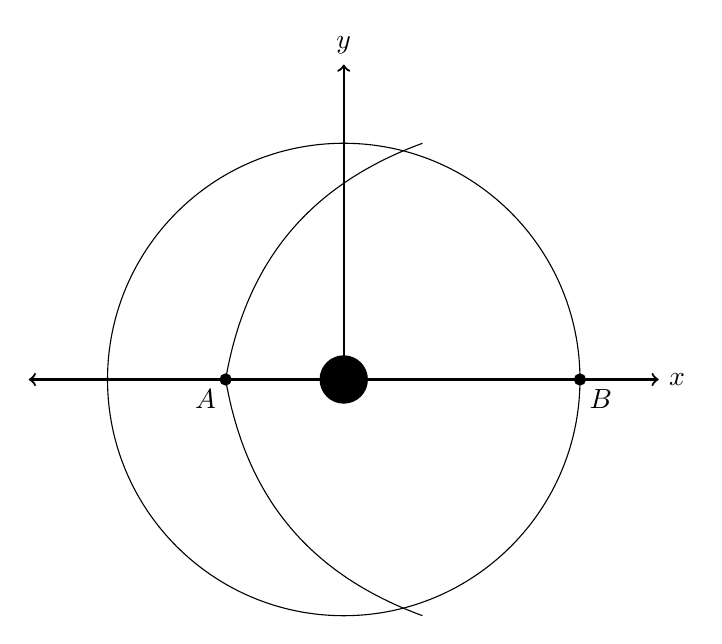
\begin{tikzpicture}
        \draw [<->, thick] (0, 4) node (yaxis) [above] {$y$} |- (4, 0) node (xaxis) [right] {$x$};
        \draw [<-, thick] (-4, 0) {} -- (0, 0) {}; 
        \draw[black, fill=black] (0, 0) circle (3mm);
        \draw[black] (0, 0) circle (3cm);
        \draw[black, fill=black] (3, 0) circle[radius=2pt] node (B) [below right] {$B$};

        % hyperbolic orbit
        \draw[black, fill=black] (-1.5, 0) circle[radius=2pt] node (A) [below left] {$A$};
        \draw[bend left] (1, -3)  to (-1.5, 0);
        \draw[bend left] (-1.5, 0) to (1, 3);
    \end{tikzpicture}
\end{scaletikzpicturetowidth}
\end{figure}
\begin{gather*}
r_A=7000\,\mathrm{km},\quad r_B=14000\,\mathrm{km},\quad v_{A_1}=12\,\mathrm{km/s},\quad \mu =398600\,\mathrm{km^3/s^2}.
\end{gather*}
We wish to design an orbital maneuver of the spacecraft such that a rendezvous between the spacecraft and the space station occurs at point B. 
The maneuver of the spacecraft is composed of the following orbits:

\begin{itemize}
    \item Hohmann transfer from the hyperbolic orbit to the circular orbit
    \item A phasing orbit to ensure a rendezvous at $B$ on the circular orbit
\end{itemize}

\begin{subprob}
\item Find the velocity change at point $A$, namely $\Delta V_{A}$, to transfer the spacecraft from the hyperbolic orbit to a transfer ellipse between $A$ and $B$.
\item Compute the time required to transfer from $A$ to $B$ during the Hohmann transfer.
\item Find the location of the space station when the spacecraft arrives at point $B$.
    You can assume the true anomaly for the space station is measured from the positive \( x \) axis.
   How much time is required for the space station to  return to $B$?
\item Find the period of the phasing orbit such that both the spacecraft and space station will arrive at point \( B \) at the same time.
    Find the semi-major axis $a_p$, and distance to the periapsis $r_C$ of the phasing orbit.
\item Find the velocity change at point $B$, namely $\Delta V_{B_1}$, to transfer the spacecraft from the Hohmann transfer ellipse to phasing orbit.
\item Find the velocity change at point $B$, namely $\Delta V_{B_2}$, to transfer the spacecraft from the phasing orbit onto the target circular orbit.
\item Show that the total velocity change is $\Delta V_{total} = |\Delta V_A| + |\Delta V_{B_1}| +|\Delta V_{B_2}|=4.2657\,\mathrm{km/s}$.
\end{subprob}


\end{prob}


% \subsection*{COMFIX Hand Calculations}
% \noindent The following problems should help you get started on the \texttt{COMFIX} project.
% All of the problems are referencing the first satellite obseravtion from \texttt{comfix.dat}.

% \begin{prob}
%     Recall the radar site and obseration data for satellite \num{1001} from \texttt{comfix.dat}, i.e. latitude \( = \SI{77.7}{\degree} N\), longitude \( = \SI{68.5}{\degree} W\), altitude \( = \SI{50}{\meter} \), Observation time = \( \SI{ 2454154.6376157}{\julianday}\).
%     Using this observation (the first one from the file), complete the following.
%     \begin{itemize}
%         \item Compute Greenwich Sidereal Time - \( GST \)
%         \item Compute Local Sidereal Time - \( LST \)
%         \item Draw a sketch of the problem using a view from the north pole and identify the location of the inertial \( x \) axis and the angles \( GST, LST\).
%     \end{itemize}
% \end{prob}

% \begin{prob}
%     Using the same site and time information from the previous problem, compute the position of the obseration site \( \vec r_{site} \) in both the inertial frame (ECI) and the Earth centered Earth fixed frame (ECEF).
% \end{prob}

% \begin{prob}
%     Using the same site and observation data, find the vectors \( \vec \rho_{ECI}, \dot \vec \rho_{ECI} \) which define the position and velocity of the satellite relative to the observation site in the Earth Centered Inertial frame.
% \end{prob}

% \begin{prob}
%     Finally, compute the position and velocity of the satellite, \( \vec r_{ECI}, \vec v_{ECI} \), in the Inertial frame and compute the classical orbital elements for this satellite.
% \end{prob}

% \section*{Extra Credit}

% \begin{prob}
%     Consider the following orbits:
%     \begin{figure}[htbp]
%         \centering
%         \begin{scaletikzpicturetowidth}{\textwidth}
%             \begin{tikzpicture}[dot/.style={draw,fill,circle,inner sep=1pt}]
%                 \def\a{4} % semi major axis
%                 \def\b{2} % semi minor axis
%                 \def\c{3} 
%                 \def\d{2}
%                 \def\fa{{sqrt(\a*\a-\b*\b)}}
%                 \def\fb{{sqrt(\c*\c-\d*\d}}
%                 \def\angle{-45} % angle at which X is placed
%                 % define attracting focus
%                 \draw[fill=black] (0, 0) circle[radius=4pt] node (earth) {};
%                 % Draw the large ellipse
%                 \draw ($(earth) - (\fa, 0)$) ellipse ({\a} and {\b});
%                 \draw ($(earth) + (\fb, 0)$) ellipse ({\c} and {\d});
%                 % Draw the inner lines and labels
%                 \draw[fill=black] ($(earth) -(\a, 0) - (\fa, 0)$) circle[radius=2pt] coordinate[label={left:$D$}] (D);
%                 \draw[circle,fill=black] ($(earth) +(\a, 0) - (\fa, 0)$) circle[radius=2pt] coordinate[label={right:$C$}] (C);
%                 \draw[circle,fill=black] ($(earth) + (\c, 0) + (\fb, 0)$) circle[radius=2pt] coordinate[label={right:$B$}] (B);
%                 \draw[circle,fill=black] ($(earth) - (\c, 0) + (\fb, 0)$) circle[radius=2pt] coordinate[label={left:$A$}] (A);
%             \end{tikzpicture}
%     \end{scaletikzpicturetowidth}
%     \end{figure}
%     with 
%     \begin{align*}
%         r_A = \SI{25000}{\kilo\meter} \quad r_B = \SI{40000}{\kilo\meter} \quad r_C = \SI{10000}{\kilo\meter} \quad r_D = \SI{55000}{\kilo\meter}
%     \end{align*}
%     \begin{subprob}
%         \item Find the minimum energy (\(\Delta V\)) transfer ellipse by comparing a transfer from \( A\) to \( C \) vs. a transfer from \( B \) to \(D\).
%         \item Sketch each transfer ellipse.
%         \item Calculate the time of flight for the minimum energy transfer.
%     \end{subprob}
% \end{prob}

% \begin{prob}
%     Given two circular coplanar orbits with \( r_i = \SI{8000}{\kilo\meter}\) and \( r_f = \SI{120000}{\kilo\meter}\), find the \( \Delta V \) required and time of flight for a bi-elliptic transfer with an intermediate radius of \( r_{int} = \SI{280000}{\kilo\meter}\). 
%     Compare this to the direct Hohmann Transfer manuever and discuss the trade-offs between the two methods.
% \end{prob}

% \begin{prob} 
%     Calculate the total \( \Delta V \), time of flight, and firing angles (\(\alpha\)) to transfer between circular coplanar orbits with \( r_i = \SI{10000}{\kilo\meter}\) and \( r_f = \SI{42160}{\kilo\meter}\) using a transfer ellipse having the parameters \( e = 0.75\) and \( p = \SI{15000}{\kilo\meter}\).
% \end{prob}

% \begin{prob}
%     Solve the following plane change problems.
%     \begin{subprob}
%     \item Show that the maximum obtainable simple plane change for a circular orbit where \( \Delta v = \Delta v_{escape} \) is \( \Delta i = \SI{23.9}{\degree}\).
%         The velocity change is defined as the \textbf{difference} in velocity between the circular orbit velocity and the velocity to escape from the circular orbit.
%     \item Show that the maximum obtainable simple plane for a circular orbit with \( \Delta v = v_{circular}\) is \( \Delta i = \SI{60}{\degree}\).
%     \item Determine the minimum  \( \Delta v \) required to complete the following transfer:
%         \begin{align*}
%             r_i &= \SI{8000}{\kilo\meter} &r_f &= \SI{42160}{\kilo\meter} \\
%             e_i &= 0  &e_f &= 0 \\
%             i_i &= \SI{30}{\degree} &i_f&=\SI{0}{\degree}
%         \end{align*}
%     \end{subprob}
% \end{prob}
\end{document}

